\documentclass [11pt]{book}

\author {David J. Cooper, Jr.}

\textwidth 6.5in

\topmargin 0in

\textheight 8.5in

\oddsidemargin 0in

\evensidemargin 0in

\pdfimageresolution 135

\title {Genworks GDL Tutorial}

\usepackage [dvips]{graphicx}

\usepackage [usenames, dvipsnames]{color}

\usepackage {makeidx}

\newsavebox {\boxedverb}

\makeindex 



\begin{document}



\frontmatter



\maketitle


\footnotetext{Copyright 
\copyright{} 2002, Genworks International. Duplication, by any means, in whole or in part, requires 
written consent from Genworks International.}

\tableofcontents



\mainmatter



\chapter{Introduction}

\label{chap:introduction}



\section{Knowledge Base Concepts According to Genworks}

\label{sec:knowledgebaseconceptsaccordingtogenworks}

You may have an idea from college or from textbooks that Knowledge Base Systems,
or Knowledge \emph{Based} Systems, are a broad or fuzzy set of concepts somehow related to \index{AI}AI which ``do not translate into anything practical.'' Or you may have heard jabs at the 
pretentious-sounding name, Knowledge-based Engineering as in: ``you mean as opposed to \index{Ignorance-based Engineering}Ignorance-based Engineering?'' To the contrary, we hope you will agree that our concept of a KB system is 
simple and practical, and in this tutorial our goal is to make you comfortable and 
excited about the ideas we have implemented in our flagship system, GDL/GWL. 

Our definition of a \emph{\index{Knowledge Base System}Knowledge Base System} is an object-oriented programming environment which implements the features of \emph{\index{Caching}Caching} and \emph{\index{Dependency tracking}Dependency tracking}. Caching means that once the KB has computed something, it might not need to repeat 
that computation if the same question is asked again. Dependency tracking is the flip side
of that coin --- it ensures that if a cached result is \emph{stale}, the result will be recomputed the next time it is \emph{demanded}, so as to give a fresh result.

\section{Goals for this Tutorial}

\label{sec:goalsforthistutorial}

This manual is designed as a companion to a live two-hour GDL/GWL tutorial, but you may
also be reading it on your own. In either case, the basic goals are:

\begin{itemize}

\item Get you excited about using GDL/GWL

\item Enable you to judge whether GDL/GWL is an appropriate tool for a given job

\item Arm you with the ability to argue the case for using GDL/GWL when appropriate

\item Prepare you to begin maintaining and authoring GDL/GWL applications, or porting apps
from similar KB systems into GDL/GWL.

\end{itemize}

This tutorial assumes a basic familiarity with the \index{Common Lisp}Common Lisp programming language. If you are new to Common Lisp: congratulations! You have just 
discovered an exciting and powerful new tool. Many resources are available to get you started 
in CL --- for starters, we recommend 
\underline{\index{Basic Lisp Techniques}Basic Lisp Techniques}\footnote{
\underline{BLT} is available at \texttt{http://www.franz.com/resources/educational\_resources/cooper.book.pdf}}, which was prepared by the author of this tutorial. Most of the Common Lisp used in this tutorial is covered in the first few chapters of 
\underline{Basic Lisp Techniques}, and there you will also find pointers to more exhaustive CL tutorials and reference material.

\section{What is GDL/GWL?}

\label{sec:whatisgdl/gwl?}

GDL is an acronym for the General-purpose Declarative Language. GWL is an acronym for
the Generative Web Language. GWL ships along with GDL in a layered, modular fashion. For the 
remainder of this tutorial, we will sometimes refer only to GDL, and this should usually be taken 
to mean the bundled package which includes GWL.

GDL is a superset of ANSI Common Lisp, and consists mainly of
automatic code-expanding extensions to Common Lisp implemented in the
form of macros. When you write, let's say, 20 lines in GDL, you might be
writing the equivalent of 200 lines of Common Lisp. Of course, since
GDL is a superset of Common Lisp, you still have the full power of the
CL language at your fingertips whenever you are working in GDL.

\index{compiled language!benefits of}\index{macros!code-expanding}Since GDL expands into CL, everything you write in GDL will be
compiled ``down to the metal'' to machine code with all the
optimizations and safety that the tested-and-true CL compiler
provides. This is an important distinction as contrasted to some other 
so-called KB systems on the market, which are really nothing more than 
interpreted scripting languages which often fall over with a ``thud'' when 
pushed to compute something more demanding than simple parameter-passing.

GDL can also be considered a \emph{\index{declarative}declarative} language. When you put together a GDL application, you write and think mainly
in terms of objects and their properties, and how they depend on one another in a direct
sense. You do not have to track in your mind explicitly how one object or property will ``call''
another object or propery, in what order this will happen, etc. Those details are
taken care of for you automatically by the language. 

Because GDL is object-oriented, you have all the features you would normally expect
from an object-oriented language, such as 

\begin{itemize}

\item Separation between the \emph{definition} of an object and an \emph{instance} of an object

\item High levels of data abstraction

\item The ability for one object to ``inherit'' from others

\item The ability to ``use'' an object without concern for its ``under-the-hood'' implementation

\end{itemize}

\index{object-orientation!message-passing}\index{object-orientation!generic-function}GDL supports the ``message-passing'' paradigm of object orientation, with some extensions. Since
full-blown ANSI CLOS (Common Lisp Object System) is always available as well, the Generic Function paradigm 
is supported as well. Do not be concerned at this point if you are not fully aware of the differences 
between these two paradigms\footnote{See Paul Graham's 
\underline{ANSI Common Lisp}, page 192, for an excellent discussion of the Two Models 
of Object-oriented Programming.}.

\section{Why GDL (what is GDL good for?)}

\label{sec:whygdl(whatisgdlgoodfor?)}



\begin{itemize}

\item Organizing and interrelating large amounts of information
in ways not possible or not practical using conventional languages or 
conventional relational database technology alone;

\item Evaluating many design or engineering alternatives and 
performing various kinds of optimizations within specified design
spaces;

\item Capturing the procedures and rules used to solve repetitive
tasks in engineering and other fields;

\item Applying rules to achieve intermediate and final 
outputs, which may include virtual models of wireframe, surface,
and solid geometric objects.

\end{itemize}



\section{What GDL is not}

\label{sec:whatgdlisnot}



\begin{itemize}

\item A CAD system (although it may operate on and/or generate geometric entities);

\item A drawing program (although it may operate on and/or generate geometric entities);

\item An Artificial Intelligence system (although it is an excellent environment for developing 
capabilities which could be considered as such);

\item An Expert System Shell (although one could be easily embedded within it).

\end{itemize}

Without further ado, then, let's turn the page and get started with some hands-on GDL...

\chapter{GDL Syntax}

\label{chap:gdlsyntax}



\section{Define-Object}

\label{sec:define-object}

\index{objects!defining}\emph{\index{Define-object}Define-object} is the basic macro for defining objects in GDL. An object 
definition maps directly into a Lisp (CLOS) class definition. 

The \texttt{define-object} macro takes three basic arguments:

\begin{itemize}

\item a \emph{name}, which is a symbol;

\item a \emph{\index{mixin-list}mixin-list}, which is a list of symbols naming other objects from which the current object 
will inherit characteristics;

\item a \emph{\index{specification-plist}specification-plist}, which is spliced in (i.e.\ doesn't have its own surrounding 
parentheses) after the mixin-list, and describes
the object model by specifying properties of the object (messages, contained objects, etc.)
The specification-plist typically makes up the bulk of the object definition.

\end{itemize}



Here are descriptions of the most common keywords making up the specification-plist:

\begin{description}

\item [\index{input-slots}input-slots]
specify information to be passed into the object instance when it is created.

\item [\index{computed-slots}computed-slots]
are really cached methods, with expressions to compute and return a value.

\item [\index{objects}objects]
specify other instances to be ``contained'' within this instance.

\item [\index{functions}functions]
are (uncached) functions ``of'' the object, i.e.\ they are actually methods which
discriminate on their first argument, which is the object instance upon which they are operating. 
GDL functions can also take other non-specialized arguments, just like a normal CL function.

\end{description}

Figure 
\ref{fig:object-hello} shows a simple example, which contains two input-slots, \texttt{first-name} and \texttt{last-name}, and a single computed-slot, \texttt{greeting}.
\begin{figure}
\begin{lrbox}{\boxedverb}
\begin{minipage}{\linewidth}

\begin{verbatim}


 (define-object hello ()
   :input-slots (first-name last-name)

   :computed-slots 
   ((greeting (format nil "Hello, ~a ~a!!" 
                     (the first-name) 
                     (the last-name)))))

\end{verbatim}
\end{minipage}
\end{lrbox}
\fbox{\usebox{\boxedverb}}

\caption{Example of Simple Object Definition}

\label{fig:object-hello}

\end{figure}
As you can see, a GDL Object is analogous in some ways to a \texttt{defun}, where the input-slots are like arguments to the function, and the computed-slots
are like return-values. But seen another way, each attribute in a GDL object is like a function in its own right.

The referencing macro \texttt{\index{the}the} shadows CL's \texttt{the} (which is a seldom-used type declaration operator). \texttt{The} in GDL is a macro which is used to reference the value of other messages 
within the same object or within contained objects. In the above example, we are using \texttt{the} to refer to the values of the messages (input-slots) named \texttt{first-name} and \texttt{last-name}. 

Note that messages used with \texttt{the} are given as symbols. These symbols are unaffected by the current Lisp \texttt{*package*}, so they can be specified either as plain unquoted symbols or as keyword
symbols (i.e.\ preceded by a colon), and the \texttt{the} macro will process them appropriately.

\section{Making Instances and Sending Messages}

\label{sec:makinginstancesandsendingmessages}

Once we have defined an object such as the example above, we can use
the constructor function \texttt{\index{make-object}make-object} in order to create an \emph{instance} of it. This function is very similar to the CLOS \texttt{\index{make-instance}make-instance} function. Here we create an instance of \texttt{hello} with specified values for \texttt{first-name} and \texttt{last-name} (the required input-slots), and assign this instance as the value of the symbol \texttt{my-instance}:

\begin{verbatim}
 GDL-USER(16): (setq my-instance
                 (make-object 'hello :first-name "John" 
                                     :last-name "Doe"))
 #<HELLO @ #x218f39c2>
\end{verbatim}As you can see, keyword symbols are used to ``tag'' the input values, and the return value is an instance of class \texttt{hello}. Now that we have an instance, we can use the macro \texttt{\index{the-object}the-object} to send messages to this instance:

\begin{verbatim}
 GDL-USER(17): (the-object my-instance greeting)
 "Hello, John Doe!!"
\end{verbatim}\texttt{The-object} is similar to \texttt{the}, but as its first argument it takes an expression which evaluates to an
object instance. \texttt{The}, by contrast, assumes that the object instance is the lexical variable \texttt{\index{self}self}, which is automatically set within the lexical context of a \texttt{define-object}.

Like \texttt{the}, \texttt{the-object} evaluates all but the first of its arguments as package-immune symbols,
so although keyword symbols may be used, this is not a requirement, and plain,
unquoted symbols will work just fine.

For convenience, you can also set \texttt{self} manually at the CL Command Prompt, and use \texttt{the} instead of \texttt{the-object} for referencing:

\begin{verbatim}
 GDL-USER(18): (setq self 
                 (make-object 'hello :first-name "John" 
                                     :last-name "Doe"))
 #<HELLO @ #x218f406a>

 GDL-USER(19): (the greeting)
 "Hello, John Doe!!"
\end{verbatim}In actual fact, \texttt{(the ...)} simply expands into \texttt{(the-object self ...)}.

\section{Objects}

\label{sec:objects}

\index{objects}\index{containment!object}\index{objects!child}\index{objects!contained}The \texttt{:objects} keyword specifies a list of ``contained'' instances,
where each instance is considered to be a ``child'' object of the current
object. Each child object is of a specified type, which itself must be defined
with \texttt{define-object} before the child object can be instantiated.

Inputs to each instance are specified as a plist of keywords and
value expressions, spliced in after the object's name and type
specification. These inputs must match the inputs protocol (i.e.\ the input-slots)
of the object being instantiated. Figure 
\ref{fig:object-city} shows an example of an object which contains some child objects.
\begin{figure}
\begin{lrbox}{\boxedverb}
\begin{minipage}{\linewidth}

\begin{verbatim}


 (define-object city ()
   :computed-slots
   ((total-water-usage (+ (the hotel water-usage)
                          (the bank water-usage))))
   :objects
   ((hotel :type 'hotel
           :size :large)
    (bank  :type 'bank
           :size :medium)))

\end{verbatim}
\end{minipage}
\end{lrbox}
\fbox{\usebox{\boxedverb}}

\caption{Object Containing Child Objects}

\label{fig:object-city}

\end{figure}
In this example, \texttt{hotel} and \texttt{bank} are presumed to be already (or soon to be) defined as objects themselves, 
which each answer the \texttt{water-usage} message. The \emph{\index{reference chains}reference chains}:

\begin{verbatim}(the hotel water-usage)
\end{verbatim} and 

\begin{verbatim}(the bank water-usage)
\end{verbatim} provide the mechanism to access messages within the child object instances.

These child objects become instantiated \emph{on demand}, meaning that the first time these instances or any of their messages
are referenced, the actual instance will be created \emph{and} cached for future reference.
\begin{figure}
\begin{lrbox}{\boxedverb}
\begin{minipage}{\linewidth}

\begin{verbatim}


 (defparameter *presidents-data*
     '((:name 
        "Carter"
        :term 1976)
       (:name "Reagan"
        :term 1980)
       (:name "Bush"
        :term 1988)
       (:name "Clinton"
        :term 1992)))
       
 (define-object presidents-container ()

   :input-slots
   ((data *presidents-data*))

   :objects
   ((presidents :type 'president
                :sequence (:size (length (the data)))
                :name (getf (nth (the-child index) (the data)) :name)
                :term (getf (nth (the-child index) (the data)) :term))))

\end{verbatim}
\end{minipage}
\end{lrbox}
\fbox{\usebox{\boxedverb}}

\caption{Sample Data and Object Definition to Contain U.S. Presidents}

\label{fig:object-presidents-container}

\end{figure}


\section{Sequences of Objects and Input-slots with a Default Expression}

\label{sec:sequencesofobjectsandinput-slotswithadefaultexpression}

Objects may be \emph{sequenced}\index{Objects!sequenced}\index{sequences}\index{object sequences}, to specify, in effect, an array or list of object instances. The most
common type of sequence is called a \emph{fixed size} sequence. See Figure 
\ref{fig:object-presidents-container} for an example of an object which contains a sequenced set of 
instances representing U.S. presidents. Each member of the sequenced set 
is fed inputs from a list of plists, which simulates a relational database 
table (essentially a ``list of rows'').
        
Note the following from this example:

\begin{itemize}

\item In order to sequence an object, the input keyword \texttt{:sequence} is added, with a list consisting of the keyword \texttt{\index{:size}:size} followed by an expression which must evaluate to a number.

\item In the input-slots, \texttt{data} is specified together with a default expression. Used this way, 
input-slots function as a hybrid of computed-slots and input-slots, allowing a \emph{default expression} as with computed-slots, but allowing a value to be passed in on 
instantiation or from the parent, as with an input-slot which has no default expression. 
A passed-in value will override the default expression.

\end{itemize}



\section{Summary}

\label{sec:summary}

This GDL syntax overview has been kept purposely brief, covering the fundamentals of the language
in a dense manner. On one hand, it is not meant to be a comprehensive language reference; on the other
hand, do not be concerned if you are still unsure about some of the terminology. The upcoming examples 
will revisit and further expand many of the topics covered here, and at some point a coherent picture 
should begin to emerge.

At that point it will be like riding a bicycle, and there will be no going back.



\chapter{GWL Syntax}

\label{chap:gwlsyntax}

\index{web user interface!creating}\index{HTTP}\index{HTML}GWL (Generative Web Language) consists essentially of a set of mixins and
a few functions which provide a convenient mechanism to present KB objects
defined in GDL through a standard HTTP/HTML web user interface. GWL ships
as a standard component of the commercial GDL product, and is available
on the GDL Trial Edition CD as well. 

GWL is designed to operate in conjunction with AllegroServe\index{AllegroServe}\index{htmlgen}\footnote{AllegroServe is an open-source webserver from Franz Inc, available
at http://opensource.franz.com} and its companion HTML generating facility, htmlgen. 

This chapter describes basic GWL usage and syntax. It assumes familiarity with the
underlying base language, GDL, covered in the previous chapter.

\section{Testing your GWL Installation}

\label{sec:testingyourgwlinstallation}

After you have installed according to \texttt{install.htm}:

\begin{enumerate}

\item Make sure you have started AllegroServe with:

\begin{verbatim}(net.aserve:start :port 9000)
\end{verbatim}(or any port of your choice)

\item In any standard web browser, go to:

\begin{verbatim}http://<hostname>:<port>/demos/robot
\end{verbatim}e.g.: 

\begin{verbatim}http://localhost:9000/demos/robot
\end{verbatim}

\end{enumerate}

You should see a page with a simple robot assembly made from boxes. If 
the robot shows up as well as the orange graphical "compass" below the 
graphics viewport, your installation is likely working correctly.

\section{GWL:Define-Package}

\label{sec:gwl:define-package}

The macro \texttt{gwl:define-package} is provided for setting up new working GWL packages.

Example:

\begin{verbatim}(gwl:define-package :gwl-user)
\end{verbatim}The \texttt{:gwl-user} package is an empty, pre-defined package for your use if you 
do not wish to make a new package just for scratch work.

For real projects it is recommended that you make and work in your
own GWL package.

\section{Basic Usage}

\label{sec:basicusage}

To present a GDL object instance as a web page requires two simple
steps:

\begin{enumerate}

\item mix in \texttt{\index{base-html-sheet}base-html-sheet} or a subclass thereof

\item define a function in the object called \texttt{\index{write-html-sheet}write-html-sheet}

\end{enumerate}

The \texttt{write-html-sheet} function should typically make use of the htmlgen \texttt{html} macro. It does not need to take any arguments.

Please see the htmlgen documentation (at \texttt{http://opensource.franz.com}, with the AllegroServe distribution, or in \texttt{<gdl-home>/doc/aserve/}) for full details on the use of htmlgen.

The code for a simple example object with its \texttt{write-html-sheet} presentation function is shown in Figure 
\ref{code:basic-usage}. This example contains two optional input slots with 
values for Name and Term of a president, and creates a simple HTML 
table displaying this information. As outlined above, in order to 
make an instance and display this object through a web browser, you 
would visit the URI:

\begin{verbatim}http://<host>:<port>/make?object=gwl-user::president
\end{verbatim}
\begin{figure}
\begin{lrbox}{\boxedverb}
\begin{minipage}{\linewidth}

\begin{verbatim}


 (define-object president (base-html-sheet)
   :input-slots
   ((name "Carter")
    (term 1976))

   :functions
   ((write-html-sheet 
     ()
     (html
      (:html
       (:head (:title (format nil "Info on President: ~a" (the name))))
       (:body 
        (:table
         (:tr (:td "Name") (:td "Term"))
         (:tr (:td (:princ (the name))) (:td (:princ (the term)))))))))))
    
\end{verbatim}
\end{minipage}
\end{lrbox}
\fbox{\usebox{\boxedverb}}

\caption{Basic Usage}

\label{code:basic-usage}

\end{figure}


\section{Page Linking}

\label{sec:pagelinking}

Creating hypertext links to other pages in the page hierarchy is
usually accomplished with the built-in GDL function of \texttt{base-html-sheet} called \texttt{write-self-link}. This GDL function, when called on a particular page instance, will write 
a hypertext link referring to that page instance.

These hypertext links are published by AllegroServe ``on the fly'' (as
a side-effect of being demanded), and are made up from the unique
root-path of the target object, as well as an \index{instance-id}instance-id which identifies the particular object instance which is the ``root'' of
the relevant page hierarchy. This is necessary because GWL maintains a
table of root-level instances. Each root-level instance will usually
correspond to one "user" or session. However, in general, there can
be a many-to-many relationship between user sessions and root-level
instances.

The instance-id is generated randomly. On a publicly-accessible website,
the maximum instance-id should be set to a very large number to decrease
the likelihood of a malicious visitor being able to ``guess'' the 
instance-id of another user. The maximum is set with the parameter \texttt{\index{gwl:*max-id-value*}gwl:*max-id-value*}. 

Figures 
\ref{code:page-linking} and 
\ref{code:link-target} show the code for making a page with a list of links
to pages representing individual U.S. presidents, resulting in a 
web page which should resemble Figure 
\ref{fig:presidents-container}. Note the call
to the \texttt{write-self-link} function inside the \texttt{dolist} in Figure 
\ref{code:page-linking}. This results in an HTML list item being generated with a hyperlink
for each ``president'' child object.

Note also the use of the \texttt{\index{write-back-link}write-back-link} function in \texttt{presidents-display}. This will generate a link back to the \texttt{\index{return-object}return-object} of the object, which defaults to the object's \texttt{parent}.
\begin{figure}
\begin{lrbox}{\boxedverb}
\begin{minipage}{\linewidth}

\begin{verbatim}


 (define-object presidents-container (base-html-sheet)
   :input-slots
   ((data '((:last-name "Carter" :term 1976)
            (:last-name "Clinton" :term 1992))))
   :objects
   ((presidents :type 'president-display
                :sequence (:size (length (the data)))
                :last-name (getf (nth (the-child index)
                                      (the data))
                                 :last-name)
                :term (getf (nth (the-child index)
                                 (the data))
                            :term)))
   :functions
   ((write-html-sheet 
     ()
     (html
      (:html
       (:head (:title "Links to Presidents"))
       (:body
        (:h1 "Links to the Presidents")
        (:ol
         (dolist (president (list-elements (the presidents)))
           (html
            (:li (the-object president (write-self-link))))))))))))
 
\end{verbatim}
\end{minipage}
\end{lrbox}
\fbox{\usebox{\boxedverb}}

\caption{Making a List of Links}

\label{code:page-linking}

\end{figure}

\begin{figure}
\begin{lrbox}{\boxedverb}
\begin{minipage}{\linewidth}

\begin{verbatim}

 
 (define-object president-display (base-html-sheet)
   :input-slots
   (last-name term)

   :computed-slots
   ((strings-for-display (the last-name)))
  
   :functions
   ((write-html-sheet
     ()
     (html
      (:html
       (:head (:title (:princ (the last-name))))
       (:body
        (:h1 (:princ (the last-name)))
        "Term: " (:princ (the term))
        (:p (the (write-back-link)))))))))

\end{verbatim}
\end{minipage}
\end{lrbox}
\fbox{\usebox{\boxedverb}}

\caption{Link Target}

\label{code:link-target}

\end{figure}

\begin{figure}
\begin{center}
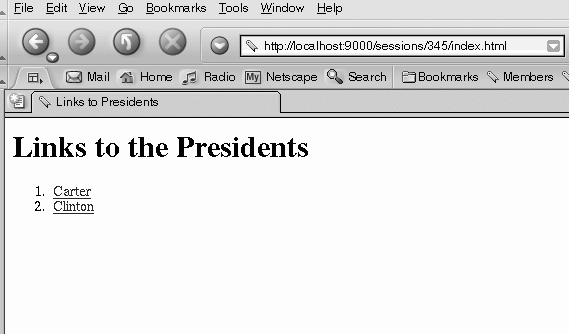
\includegraphics{../images/presidents-container.png}
\end{center}

\caption{Presidents Container Page with Links}

\label{fig:presidents-container}

\end{figure}


\section{Form Handling}

\label{sec:formhandling}

\index{form handling}Forms are generated using the GWL macro\texttt{with-html-form}. You wrap this macro around the HTMLgen code which creates the contents of the form:

\begin{verbatim}

 (with-html-form ()
  
   ;; the body of your form goes here
  
    )
\end{verbatim}The above code snippet would be included in a \texttt{write-html-sheet}function of a page definition.  

By default, the same object which
generates the form will also respond to the form, and is also the
object which will have its settable slots modified based on form
fields (i.e. html ``inputs'') of the same name. You can override the
default by specifying a \texttt{bashee} and/or \texttt{respondent}as slots in the requestor object (i.e. the object which is generating the form), for
example:

\begin{verbatim}

 :computed-slots
 ((respondent (the some-other-object))
  (bashee (the yet-another-object)))


\end{verbatim}Any \texttt{:settable} computed-slots in the object may be specified as input values (i.e.\ with \texttt{:input} tags) in the form. GWL will automatically infer their types
and do appropriate conversion. If the type of a slot can vary, it is best
to make its default be a string, then have your application read from
the string (with the \texttt{\index{read-safe-string}read-safe-string} function).

Note that only those input values which have actually changed
 (according to \texttt{equalp} ) will be set into the corresponding computed-slot upon form submission. 
Ones which remain the same will be left alone (to avoid unnecessary dependency 
updating in the model).

Any \texttt{:input} values in the form whose name does not match one of the \texttt{:settable} computed-slots in the object will still be collected, but rather than being set into
 its own named slot, it will be returned as part of the special \texttt{query-plist} message when the response page's \texttt{write-html-sheet} method is invoked. \texttt{Query-plist} is a plist containing keywords representing the form field names, and 
values which will be strings representing the submitted values.


If you want to do additional processing, the following functions are provided
for \texttt{base-html-sheet}:

\begin{description}

\item [before-set!]
This is invoked before the ``bashee'' is modified with any new form values.

\item [after-set!]
This is invoked after the ``bashee'' is modified with any new form values.

\item [before-present!]
This is invoked after the ``bashee'' is modified with any new form values, but 
before the page content is returned to the web client.

\item [after-present!]
This is invoked after the page content is returned to the web client.

\end{description}

 By default, these functions are empty, but you can override them to do whatever 
extra processing you wish.

Figure 
\ref{code:hello-form} shows an object which both generates and responds to a simple form,
with the corresponding web page shown in Figure 
\ref{fig:hello-form}. The form allows the user to type a name to override the default ``Jack,'' and 
reflects the submitted name in the form page upon response.

To instantiate this object in a web browser, you would visit the URI:

\begin{verbatim}http://<host>:<port>/make?object=gwl-user::hello-form
\end{verbatim}
\begin{figure}
\begin{lrbox}{\boxedverb}
\begin{minipage}{\linewidth}

\begin{verbatim}


 (define-object hello-form (base-html-sheet)

   :computed-slots ((username "Jack" :settable))

   :functions
   ((write-html-sheet 
     ()
     (html
      (:html 
       (:head (:title "Sample Form"))
       (:body 
        (:p "Hello there, " (:princ (the username)) "!")
        (:p (with-html-form ()
             ((:input :type :text :name :username 
                      :value (the username)))
             ((:input :type :submit :name :submit 
                      :value " Change Name! "))))))))))

\end{verbatim}
\end{minipage}
\end{lrbox}
\fbox{\usebox{\boxedverb}}

\caption{Hello Form}

\label{code:hello-form}

\end{figure}

\begin{figure}
\begin{center}
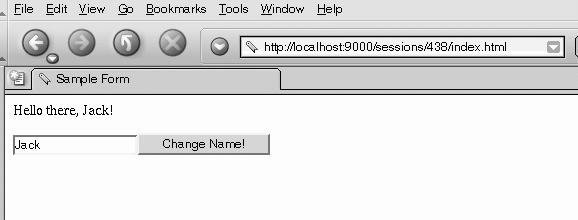
\includegraphics{../images/hello-form.png}
\end{center}

\caption{Hello Form}

\label{fig:hello-form}

\end{figure}


\section{Publishing URIs for GWL Objects}

\label{sec:publishingurisforgwlobjects}

\index{publishing!of GWL URIs}You can publish a URI for a given object, to avoid having to type the
``make?'' expression, using the AllegroServe \texttt{publish} function and the GWL \texttt{\index{gwl-make-object}gwl-make-object} function, as per the following example:

\begin{verbatim}
  (publish :path "/demos/bus"
           :function #'(lambda(req ent)
                         (gwl-make-object req ent "bus:assembly")))
\end{verbatim}In this example, the ``bus'' object would now be instantiated simply by
visiting the URI:

\begin{verbatim}http://<host>:<port>/bus
\end{verbatim}

\section{Higher-level Apps and Graphics}

\label{sec:higher-levelappsandgraphics}

GDL/GWL also has the ability to generate and display standard wireframe geometric
entities. The complete list of currently available primitive geometric objects is available
in the GDL documentation set. Currently the only documented way to display geometry in
a GWL application is by using the higher-level mixin \texttt{\index{application-mixin}application-mixin}. Two complete examples of the use of this mixin, the Robot and the School Bus, are
given in Chapters 
\ref{chap:example2:simplifiedandroidrobot} and 
\ref{chap:example3:schoolbus}. Here we will just touch on the basics of how to use this
mixin.

\begin{enumerate}

\item Instead of \texttt{base-html-sheet}, mix in \texttt{application-mixin} into the object definition you wish to publish via the web.

\item Collect the objects whose leaves you wish to display as geometry in a computed-slot named\texttt{\index{ui-display-list-objects}ui-display-list-objects}.

\end{enumerate}

Following the above steps will result in a page with a default user interface which 
will display your graphics in the center. This page, and each of its components, are highly
customizable, and we will look at some of the available customizations in the examples in
Chapters 
\ref{chap:example2:simplifiedandroidrobot} and 
\ref{chap:example3:schoolbus}.

\chapter{Example 1: Personal Ledger}

\label{chap:example1:personalledger}

In this chapter we will describe a simple personal accounting ledger application. 
First we will build the core objects necessary to keep track of accounts and transactions; 
then we will layer a web user interface on top of these objects to allow for convenient
end-user access. 

I have chosen to build this application in base GDL/GWL, without the use of any database\footnote{\index{Paul Graham}Paul Graham is fond of reminding us that ``the filesystem is already a database.''} or other general-purpose mixins. Clearly, one could greatly reduce the amount of code
required for an application like this by using ``utility'' mixins for tasks such as database or
filesystem access and standard GUI templates. 

While it certainly does not implement the most efficient accounting/ledger algorithms possible, 
this application will give us a small taste of the power of the caching and dependency-tracking
features of a KB system.

\section{Main Ledger Object}

\label{sec:mainledgerobject}

The full source for the Ledger application is available in the GDL application directory under the \texttt{gwl-samples} directory. We include partial hardcopy in this tutorial, but if you wish to try running the example 
yourself you should use the code from the CD rather than trying to type it in from this hardcopy (also, 
some changes may have occured since the preparation of this tutorial). 

The ledger application needs write access to files under the \texttt{gwl-samples/ledger/data/} directory, so you may need to open up permissions on these files, or copy the entire \texttt{ledger/} directory to a location where you have write access, such as your home directory. 

Figure 
\ref{code:ledger-input-computed} shows the input-slots and computed-slots of our main object, named conventionally 
``assembly'' (in the \texttt{:ledger} Lisp package). The two inputs each default to a file holding the beginning 
data set for Accounts and Transactions respectively. Figure 
\ref{data:ledger-data} shows a sampling of the first few lines from typical data files. 
These data files are given the ``lisp'' extension simply so that they will 
come up in Lisp-mode in Emacs for ease of hand-editing -- they are not
meant to be compiled as Lisp program source code.

The \texttt{account-data} and \texttt{transaction-data} computed-slots read and hold the contents of these data files for use in 
initializing the actual \texttt{accounts} and \texttt{transactions} object sequences, which the ledger application will use. The \texttt{account-indices} and \texttt{transaction-indices} collect up the unique indices from the individual acounts and transactions, 
used to compute the ``next'' index when adding a new ``record.'' The \texttt{net-worth} and \texttt{profit} slots compute the sums of Asset/Liability accounts and Income/Expense accounts, 
respectively (the sign on \texttt{profit} is reversed to make Income items appear positive and 
Expense items appear negative). Finally, the \texttt{balances-hash-table} slot is a hash table keyed on the account indices, computing the current balance
of each account. This value is passed into the actual account objects for later use.
\begin{figure}
\begin{lrbox}{\boxedverb}
\begin{minipage}{\linewidth}

\begin{verbatim}


 ("Index" "Name" "Description" "Account Number" 
  "Account Type" "Account Class" "Beginning Balance") 
 (0 "DFCU" "Dearborn Federal Credit Union" "999-6969-999" 
  "Checking" "Asset/Liability" 25000) 
 (1 "Waterhouse" "Waterhouse Taxable" "555-7979-555" 
  "Savings" "Asset/Liability" 12500) 

   ...


 ("Index" "From Account" "To Account" "Date" "Amount" "Payee") 
 (0 0 1 3243976597 1000 "djc") 
 (1 0 1 3243976772 1500 "djc")

   ...

\end{verbatim}
\end{minipage}
\end{lrbox}
\fbox{\usebox{\boxedverb}}

\caption{Contents of Account and Transaction Data Files}

\label{data:ledger-data}

\end{figure}

\begin{figure}
\begin{lrbox}{\boxedverb}
\begin{minipage}{\linewidth}
\small{}
\end{minipage}
\end{lrbox}
\fbox{\usebox{\boxedverb}}

\caption{Input-Slots and Computed-Slots of Ledger}

\label{code:ledger-input-computed}

\end{figure}
Figure 
\ref{fig:genacc2-subobjects} shows the two sub-objects contained within the ledger assembly object. Each of these
is specified as a \texttt{\index{sequence}sequence}, based on the initial data read from the data files. Because these sequences are specified
by a list of \texttt{\index{:indices}:indices}, rather than by a fixed \texttt{\index{:size}:size}, they can be programmatically modified by inserting and deleting sequence elements. In 
this example, such insertions or deletions would be analogous to row operations on a relational
database table. 

Note that the \texttt{current-balance} is accessed from the \texttt{balances-hash-table}, a computed-slot listed in Figure 
\ref{code:ledger-input-computed}.
\begin{figure}
\begin{lrbox}{\boxedverb}
\begin{minipage}{\linewidth}
\small{

\begin{verbatim}


    ...
       
  :objects
  ((accounts :type 'account
             :sequence (:indices (mapcar #'first (rest (the account-data))))
             :data (nth (the-child index) (rest (the account-data)))
             :current-balance (gethash (the-child index) 
                                       (the balances-hash-table))
             :headings (first (the account-data)))
   
   (transactions :type 'transaction
                 :sequence (:indices (mapcar #'first 
                                             (rest (the transaction-data))))
                 :data (nth (the-child index) (rest (the transaction-data)))
                 :headings (first (the transaction-data))))
  

    ...

\end{verbatim}}
\end{minipage}
\end{lrbox}
\fbox{\usebox{\boxedverb}}

\caption{Sub-Objects of Ledger}

\label{fig:genacc2-subobjects}

\end{figure}
The final segment of our main ledger object is listed in Figure 
\ref{fig:genacc2-functions}. Here, we specify some functions on the ledger object which accept
arguments and perform some side-effect on the object. Note that GDL \texttt{:functions} are distinguished from \texttt{:computed-slots} by two main characteristics:

\begin{enumerate}

\item They can accept arguments, a ``lambda list,'' as with a normal CL function.

\item Their return-values are not cached or dependency-tracked. Their bodies are 
evaluated every time they are referenced (called).

\end{enumerate}

The \texttt{add-transaction!} function adds a new transaction element to the \texttt{transactions} object sequence, and immediately calls the \texttt{save-transactions!} function to update the transactions data file\footnote{In a more robust application, the in-memory insertion and
the updating of the external file should be done as an indivisible unit 
with ``unwind'' capability, to ensure that either the whole thing succeeds 
or the whole thing fails.}. 

The most important thing to note here is that when a new transaction is added
using the \texttt{add-transaction!} function, any other message (e.g. computed-slot, object, etc.) which in any
way depends upon the \texttt{transactions}\index{recomputation!on-demand} sequence of objects will now automatically recompute and return a fresh
value the next time it is demanded. For example, the \texttt{profit} and \texttt{net-worth} messages will now return updated values the next time they are demanded.
But the recomputation of a message will happen if and only if the message is
actually demanded. In a very large object tree, for example, thousands of messages
in hundreds of objects might depend on a certain value. 

When that value is 
changed, however, the system 
\underline{does not} incur the computational overhead of 
updating all these thousands of dependent items at that time. Perhaps only a 
few dozen of these thousands of dependent items will ever be accessed. Only 
those few dozen will need to be computed.

This is one of the obvious distinctions between a conventional ``spreadsheet'' 
application and a knowledge base application --- a spreadsheet is generally not 
scalable to very large problems or models, because changing a value forces the 
user to wait for an all-or-nothing update of the entire sheet.\index{spreadsheet!KB as distinct from}
\begin{figure}
\begin{lrbox}{\boxedverb}
\begin{minipage}{\linewidth}
\small{

\begin{verbatim}


   ...

  :functions
  ((add-transaction! (&key from-account to-account date amount payee)
    (when (or (not (member from-account (the account-indices)))
              (not (member to-account (the account-indices)))
              (not (numberp amount)) (not (stringp payee))
              (not (ignore-errors (decode-universal-time date))))
      (error "One or more invalid arguments given to add-transaction!"))
    (let ((new-index (1+ (if (null (the transaction-indices)) 0 
                           (apply #'max (the transaction-indices))))))
      (the transactions (insert! new-index))
      (the (transactions new-index) 
        (set-slot! :data (list new-index from-account 
                               to-account date amount payee))))
    (the save-transactions!))
   
   (save-transactions! ()
    (with-open-file (out (the transaction-data-file) 
                     :direction :output :if-exists :supersede 
                     :if-does-not-exist :create)
      (print (first (the transaction-data)) out)
      (dolist (transaction (list-elements (the transactions)))
        (print (the-object transaction data) out))))

   
      ;; ... Similarly for add-account! and save-accounts!

   )))

\end{verbatim}}
\end{minipage}
\end{lrbox}
\fbox{\usebox{\boxedverb}}

\caption{Functions of Ledger}

\label{fig:genacc2-functions}

\end{figure}


\section{Objects for Accounts and Transactions}

\label{sec:objectsforaccountsandtransactions}

Figure 
\ref{fig:genacc2-accountandtransaction} shows the object definitions for \texttt{account} and \texttt{transaction}. These are simple objects which essentially receive some inputs and make them
available as messages.
\begin{figure}
\begin{lrbox}{\boxedverb}
\begin{minipage}{\linewidth}

\begin{verbatim}


 (define-object account (base-object)
   :input-slots
   (data headings current-balance)
  
   :computed-slots
   ((name (second (the data)))
    (description (third (the data)))
    (account-number (fourth (the data)))
    (account-type (fifth (the data)))
    (account-class (sixth (the data)))
    (beginning-balance (seventh (the data)))))

 (define-object transaction (base-object)
   :input-slots
   (data headings)
  
   :computed-slots
   ((from-account (second (the data)))
    (to-account (third (the data)))
    (date (fourth (the data)))
    (amount (fifth (the data)))
    (payee (sixth (the data)))))

\end{verbatim}
\end{minipage}
\end{lrbox}
\fbox{\usebox{\boxedverb}}

\caption{Account and Transaction Object Definitions}

\label{fig:genacc2-accountandtransaction}

\end{figure}


\section{Using the Main Ledger Object}

\label{sec:usingthemainledgerobject}

We can use the ledger object we have put together so far by typing commands at the 
Common Lisp prompt. First, we will make an instance of a ledger object, conveniently 
setting this instance to the variable \texttt{self}:

\begin{verbatim}
LEDGER(10): (setq self (make-object 'assembly))
#<ASSEMBLY @ #x7367516a>
\end{verbatim}Now we can use ``the'' referencing to call various messages in this instance:

\begin{verbatim}
LEDGER(11): (the profit)
140
LEDGER(12): (the net-worth)
37640
LEDGER(13): (the balances-hash-table)
#<EQL hash-table with 7 entries @ #x7367fc1a>
LEDGER(14): (the (accounts 0) current-balance)
28140
LEDGER(15):
\end{verbatim}Now we will add a transaction, and confirm that it affects our \texttt{profit} and \texttt{net-worth}:

\begin{verbatim}
LEDGER(15): (the (add-transaction! :from-account 0 :to-account 4 
                                   :date (get-universal-time) 
                                   :amount 250 :payee "djc"))
NIL
LEDGER(16): (the profit)
-110
LEDGER(17): (the net-worth)
37390
LEDGER(18):
\end{verbatim}If we had wrapped the CL \index{time!using to understand KB dynamics}\texttt{time} macro around for example the call to the \texttt{profit}, we would have been able to see that indeed it was recomputed the second time
we called it, since something it depends upon had been modified. If we call it again
immediately, without having changed anything, \texttt{time} would show us that it returns virtually instantaneously without causing any
substantial work to be done, since its value is now cached and the cache is still fresh.

\section{Making a Web Interface with GWL}

\label{sec:makingawebinterfacewithgwl}

Now that we have built and tested our main ledger ``engine,'' let's make it more 
accessible to casual users by layering a web user interface on it. One way to do this is
to create a new toplevel object which \emph{contains} the ledger engine, and specifies an assembly of objects to represent the web
pages in our interface. Figure 
\ref{code:ledger-html-top} shows the definition of the top level, or ``home page,'' of our web application.
 
It contains the actual ledger assembly, or ``engine,'' as well as child objects, which
represent sub-pages in our website, corresponding to an account listing, a transaction
listing, a form for adding a transaction, and a form for adding an account.
\begin{figure}
\begin{lrbox}{\boxedverb}
\begin{minipage}{\linewidth}

\begin{verbatim}


 (define-object html-assembly (base-html-sheet)
  
   :computed-slots 
   ((accounts-ht (let ((ht (make-hash-table)))
                   (dolist (account (list-elements 
                                     (the ledger accounts)) ht)
                     (setf (gethash (the-object account index) ht) 
                       account)))))
  
   :objects
   ((ledger :type 'assembly)
  
    (view-accounts :type 'view-accounts
                   :account-sequence (the ledger accounts))
   
    (view-transactions :type 'view-transactions
                       :transaction-sequence (the ledger transactions)
                       :pass-down (accounts-ht))
   
    (add-transaction :type 'add-transaction
                     :main-sheet self
                     :pass-down (accounts-ht))
   
    (add-account :type 'add-account
                 :main-sheet self))
  ...

\end{verbatim}
\end{minipage}
\end{lrbox}
\fbox{\usebox{\boxedverb}}

\caption{Slots and Object for Web Interface}

\label{code:ledger-html-top}

\end{figure}
Our toplevel user interface sheet also contains a \texttt{write-html-sheet} presentation function, shown in Figure 
\ref{code:ledger-html-bottom}. This presentation function also serves as a response function
to the forms for adding accounts and transactions -- for this reason, 
it contains two blocks of code, before the actual html page generation,
which take care of actually processing any added transaction or account.

The form values for these will show up as plist values in the \texttt{query-plist} slot, since they are not specified as named slots in the 
objects which generate the forms (the transaction form is shown 
in Figure 
\ref{code:add-transactions-sheet}, and the accounts form is not listed here but is similar).
\begin{figure}
\begin{lrbox}{\boxedverb}
\begin{minipage}{\linewidth}
\small{

\begin{verbatim}


  :functions
  ((write-html-sheet
    ()
    (let ((plist (the add-transaction query-plist)))
      (when plist
        (the ledger 
          (add-transaction! 
           :from-account (read-safe-string (getf plist :from-account))
           :to-account (read-safe-string (getf plist :to-account))
           :date (iso-to-universal (getf plist :date))
           :amount (read-safe-string (getf plist :amount))
           :payee (getf plist :payee))))
      (the add-transaction (:set-slot! :query-plist nil)))
    (let ((plist (the add-account query-plist)))
      (when plist
        (the ledger (add-account! 
                     :name (getf plist :name)
                     :description (getf plist :description)
                     :account-number (getf plist :account-number)
                     :account-type (getf plist :account-type)
                     :account-class (getf plist :account-class)
                     :beginning-balance (read-safe-string 
                                         (getf plist :beginning-balance)))))
      (the add-account (:set-slot! :query-plist nil)))
    (html 
     (:html 
      (:head (:title "Personal Ledger"))
      (:body 
       (:h2 (:center "Personal Ledger"))
       (:p (:table 
            (:tr (:td "Net Worth:")
                 ((:td :align :right) 
                  (:b (:tt ((:font 
                             :color (gethash (if (minusp (the ledger net-worth)) 
                                                 :red :green-lime) *color-table*))
                            (:princ (number-format (the ledger net-worth) 2)))))))
            (:tr (:td "Profit/Loss:")
                 ((:td :align :right)
                  (:b (:tt ((:font 
                             :color (gethash (if (minusp (the ledger profit)) 
                                                 :red :green-lime) *color-table*))
                            (:princ (number-format (the ledger profit) 2)))))))))
       (:p (:ul (:li (the view-accounts 
                       (write-self-link :display-string "View Accounts")))
                (:li (the view-transactions 
                       (write-self-link :display-string "View Transactions")))
                (:li (the add-transaction 
                       (write-self-link :display-string "Add Transaction")))
                (:li (the add-account 
                       (write-self-link :display-string "Add Account")))))))))))

\end{verbatim}}
\end{minipage}
\end{lrbox}
\fbox{\usebox{\boxedverb}}

\caption{Output Function for Web Interface}

\label{code:ledger-html-bottom}

\end{figure}

\begin{figure}
\begin{center}
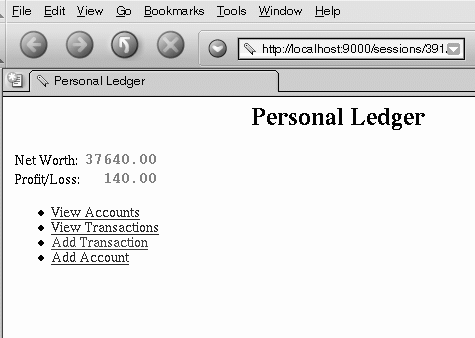
\includegraphics{../images/ledger-main.png}
\end{center}

\caption{Main Screen of Ledger}

\label{fig:ledger-main}

\end{figure}

\begin{figure}
\begin{center}
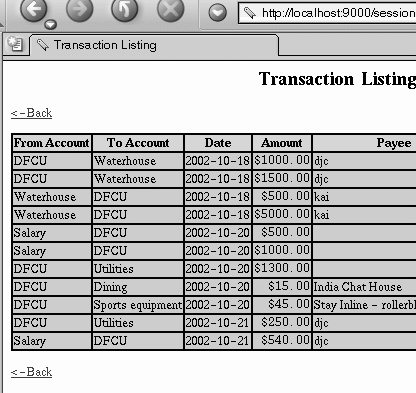
\includegraphics{../images/transaction-listing.png}
\end{center}

\caption{Transaction Listing Sheet}

\label{fig:transaction-listing}

\end{figure}
Figure 
\ref{code:view-transactions-sheet} defines an object which takes two inputs and computes 
two simple slots, but most of all it defines a presentation method to 
generate an html table listing all transactions entered to date. An example 
is seen in Figure 
\ref{fig:transaction-listing}.
\begin{figure}
\begin{lrbox}{\boxedverb}
\begin{minipage}{\linewidth}

\begin{verbatim}


 (define-object view-transactions (base-html-sheet)
   :input-slots (transaction-sequence accounts-sequence)

   :computed-slots ((transactions (list-elements 
                                   (the transaction-sequence)))
                    (headings (the-object (first (the transactions)) 
                                          headings)))
   :functions
   ((write-html-sheet
     ()
     (html 
      (:html 
       (:head (:title "Transaction Listing"))
       (:body 
        (:h2 (:center "Transaction Listing"))
        (:p (the (:write-back-link)))
        (:p ((:table :bgcolor :black)
             ((:tr :bgcolor :yellow) 
              (dolist (heading (rest (the headings)))
                (html (:th (:princ heading)))))
             (dolist (transaction (the transactions))
               (html 
                ((:tr :bgcolor (gethash :grey-light-very 
                                        *color-table*))
                 (dolist (slot (list :from-account :to-account 
                                     :date :amount :payee ))
                   (let* ((raw-value 
                           (the-object transaction (evaluate slot)))
                          (value (case slot 
                                   ((:from-account :to-account)
                                    (the :accounts-sequence 
                                      (get-member raw-value) :name))
                                   (:date (iso-date raw-value))
                                   (:amount (number-format raw-value 2))
                                   (otherwise raw-value))))
                     (html ((:td :align (case slot (:amount :right)
                                              (otherwise :left))) 
                            (case slot (:amount 
                                        (html 
                                         (:tt (format *html-stream* 
                                                      "$~$" value))))
                                  (otherwise 
                                   (html (:princ value)))))))))))))
        (:p (the (:write-back-link)))))))))

\end{verbatim}
\end{minipage}
\end{lrbox}
\fbox{\usebox{\boxedverb}}

\caption{Sheet for Transaction Listing}

\label{code:view-transactions-sheet}

\end{figure}
Figure 
\ref{code:add-transactions-sheet} defines a presentation function to create a fillout-form for adding
a transaction, and Figure 
\ref{fig:add-transaction} shows a sample rendition of this form.
\begin{figure}
\begin{lrbox}{\boxedverb}
\begin{minipage}{\linewidth}
\small{

\begin{verbatim}


 (define-object add-transaction (base-html-sheet)
   :input-slots (accounts-sequence main-sheet)

   :computed-slots ((respondent (the main-sheet)))
   
   :functions
   ((write-html-sheet
     ()
     (html 
      (:html 
       (:head (:title "Add Transaction"))
       (:body 
        (:h2 (:center "Add Transaction"))
        (:p (the (:write-back-link)))
        (with-html-form
         (:p 
          ((:table :bgcolor :black)
           (:tr 
            ((:td :bgcolor :yellow) "From Account")
            ((:td :bgcolor (gethash :green-spring *color-table*))
             ((:select :name :from-account)
              (mapcar #'(lambda(account)
                          (html ((:option 
                                  :value (the-object account index))
                                 (:princ (the-object account name)))))
                      (list-elements (the accounts-sequence))))))
           (:tr 
            ((:td :bgcolor :yellow) "To Account")
            ((:td :bgcolor (gethash :green-spring *color-table*))
             ((:select :name :to-account)
              (mapcar #'(lambda(account)
                          (html ((:option 
                                  :value (the-object account index))
                                 (:princ (the-object account name)))))
                      (list-elements (the accounts-sequence))))))
           (:tr 
            ((:td :bgcolor :yellow) "Date")
            ((:td :bgcolor (gethash :green-spring *color-table*))
             ((:input :type :text :name :date :size 12 
                      :value (iso-date (get-universal-time))))))
           (:tr ((:td :bgcolor :yellow) "Amount") 
                ((:td :bgcolor (gethash :green-spring *color-table*))
                 ((:input :name :amount :type :text :size 15))))
           (:tr ((:td :bgcolor :yellow) "Payee") 
                ((:td :bgcolor (gethash :green-spring *color-table*))
                 ((:input :name :payee :type :text :size 30))))))
         (:p ((:input :type :submit :name :add-transaction 
                      :value " Add! "))))))))))      

\end{verbatim}}
\end{minipage}
\end{lrbox}
\fbox{\usebox{\boxedverb}}

\caption{Form for Adding a Transaction}

\label{code:add-transactions-sheet}

\end{figure}

\begin{figure}
\begin{center}
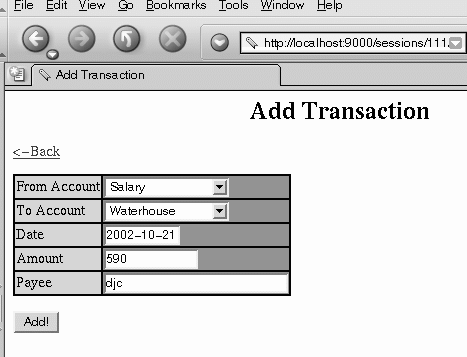
\includegraphics{../images/add-transaction.png}
\end{center}

\caption{Form for Adding a Transaction}

\label{fig:add-transaction}

\end{figure}


\section{Summary}

\label{sec:summary}


Please note that we have built this ledger using only core GDL/GWL,
for illustrative purposes. Several parts of the app have been written
from scratch, which otherwise could be handled by using simple
utilities or libraries for things such as filesystem/database access
and user interface templates.

\index{mainstream apps!KB technology useful for}\index{requirements!ever-expanding}The main point of this example is to show that KB technology can be
useful even for applications which might be considered ``simple'' or
``mainstream'' --- even the simplest of applications tend to grow
ever-changing and ever-expanding requirements, and it pays in the 
end to use a development environment which can absorb these
requirements gracefully and with ease.

\chapter{Example 2: Simplified Android Robot}

\label{chap:example2:simplifiedandroidrobot}

This chapter describes and shows the complete code for a Simplified Android Robot\footnote{The ``Simplified Android Robot'' is a traditional example used for pedagogical 
purposes in computer graphics, and as far as we know it has its origins in 
\underline{Computer Graphics: Principles and Practice} by Foley, Feiner, and Van Dam.}\index{objects!primitive!geometric} implemented in GDL/GWL. Here we introduce the use of geometric primitive objects, 
as well as the use of the higher-level \texttt{\index{application-mixin}application-mixin} first introduced in Chapter 
\ref{chap:gwlsyntax}.

We also introduce the concept of the \emph{\index{view}view}, which allows separation of presentation functions (e.g. for HTML output) from the
core object definition.

\section{Main UI Sheet for the Robot}

\label{sec:mainuisheetfortherobot}

Figure 
\ref{code:robot-toplevel} defines the toplevel user interface sheet for the robot.
It specifies several \texttt{:settable} computed-slots which the user will end up being able to set through an HTML form.
It also specifies the \texttt{robot} child object, whose leaves contain the actual geometry (boxes in this
case) of the robot.

Figure 
\ref{code:robot-model-inputs} shows the definition of a \emph{view} which is defined for the \texttt{html-format} output format, and the \texttt{robot-assembly} GDL object. Rather than being associated with a single type
as with normal GDL objects, views are associated with \emph{two} types -- an output format and a normal GDL object type. The \texttt{:output-functions} defined within the view will therefore be associated with the \emph{combination} of the given output-format and the given GDL object type. In 
this case, we are specifying the \texttt{\index{model-inputs}model-inputs} \texttt{:output-function} to be applied to the combination of the \texttt{html-format} output-format and the \texttt{robot-assembly} GDL object type.

The \texttt{application-mixin} contains a default (essentially blank) \texttt{model-inputs} function, and here we are overriding it to do something specific, namely
to display html input fields for the slots in our \texttt{robot-assembly} which we wish the user to be able to alter through a form.

By default, the \texttt{application-mixin} will display the output from the \texttt{model-inputs} function in the upper-right area of the user interface sheet, as
seen in Figure 
\ref{fig:robot}. These input fields are automatically contained inside an appropriate
HTML form entity - when using \texttt{application-mixin}, there is no need for application-level code to generate the HTML form
tag or the \texttt{\index{:respondant}:respondant} or \texttt{\index{:bashee}:bashee} hidden fields described in Chapter 
\ref{chap:gwlsyntax} with plain \texttt{\index{base-html-sheet}base-html-sheet}.
\begin{figure}
\begin{lrbox}{\boxedverb}
\begin{minipage}{\linewidth}

\begin{verbatim}


 (define-object robot-assembly (application-mixin)
  
   :computed-slots
   ((width 5 :settable)
    (length 2 :settable)
    (height 10 :settable)
    (head-angle 0 :settable)
    (body-angle 0 :settable)
    (arm-angle-right 0 :settable)
    (arm-angle-left 0 :settable)
    (pincer-distance-right (to-single-float 
                            (number-round (* .15 3/5 (the width)) 3)) 
                           :settable)
    (pincer-distance-left (to-single-float 
                           (number-round (* .15 3/5 (the width)) 3)) 
                          :settable)
    (image-format (the view-object image-format))
    (strings-for-display "Robot Assembly")
    (ui-display-list-objects (the robot)))

   :objects
   ((robot :type 'robot
           :pass-down (:head-angle 
                       :body-angle :arm-angle-right :arm-angle-left
                       :pincer-distance-right :pincer-distance-left))))

\end{verbatim}
\end{minipage}
\end{lrbox}
\fbox{\usebox{\boxedverb}}

\caption{UI Sheet for Robot}

\label{code:robot-toplevel}

\end{figure}

\begin{figure}
\begin{lrbox}{\boxedverb}
\begin{minipage}{\linewidth}
\small{

\begin{verbatim}


 (define-view (html-format robot-assembly)()
   :output-functions
   ((model-inputs
     ()
     (html 
      ((:table  :cellpadding 0)
       (:tr ((:td :colspan 2) (:b "Dimensions:")))
       (dolist (slot (list :width :length :height))
         (html 
          (:tr ((:td :bgcolor :yellow)
                (:princ (string-capitalize slot)))
               (:td ((:input :type :string :name slot :size 5
                             :value (format nil "~a" 
                                            (the (evaluate slot)))))))))
       (:tr ((:td :colspan 2) :br))
       (:tr ((:td :colspan 2) (:b "Angles:")))
       (dolist (angle '(("Head" :head-angle)("Body" :body-angle)
                        ("Left Arm" :arm-angle-left) 
                        ("Right Arm" :arm-angle-right)))
         (html
          (:tr ((:td :bgcolor :yellow) (:princ (first angle)))
               (:td ((:input 
                      :type :string :name (second angle) 
                      :size 5 :value 
                      (format nil "~a" (the (evaluate (second angle))))))))))
       (:tr ((:td :colspan 2) :br))
       (:tr ((:td :colspan 2) (:b "Grip Opening:")))
       (dolist (side (list :left :right))
         (html
          (:tr 
           ((:td :bgcolor :yellow) (:princ (string-capitalize side)))
           (:td 
            ((:input 
              :type :string 
              :name (format nil "pincer-distance-~a" side) 
              :size 5 
              :value 
              (the (evaluate (make-keyword 
                              (format nil "pincer-distance-~a" side))))))))))
       (:tr ((:td :colspan 2) :br))
       (:tr ((:td :colspan 2 :align :center)
             ((:input :type :submit :value " OK " :name :refresh)))))))))
      
\end{verbatim}}
\end{minipage}
\end{lrbox}
\fbox{\usebox{\boxedverb}}

\caption{Inputs Section for UI Sheet}

\label{code:robot-model-inputs}

\end{figure}

\begin{figure}
\begin{center}
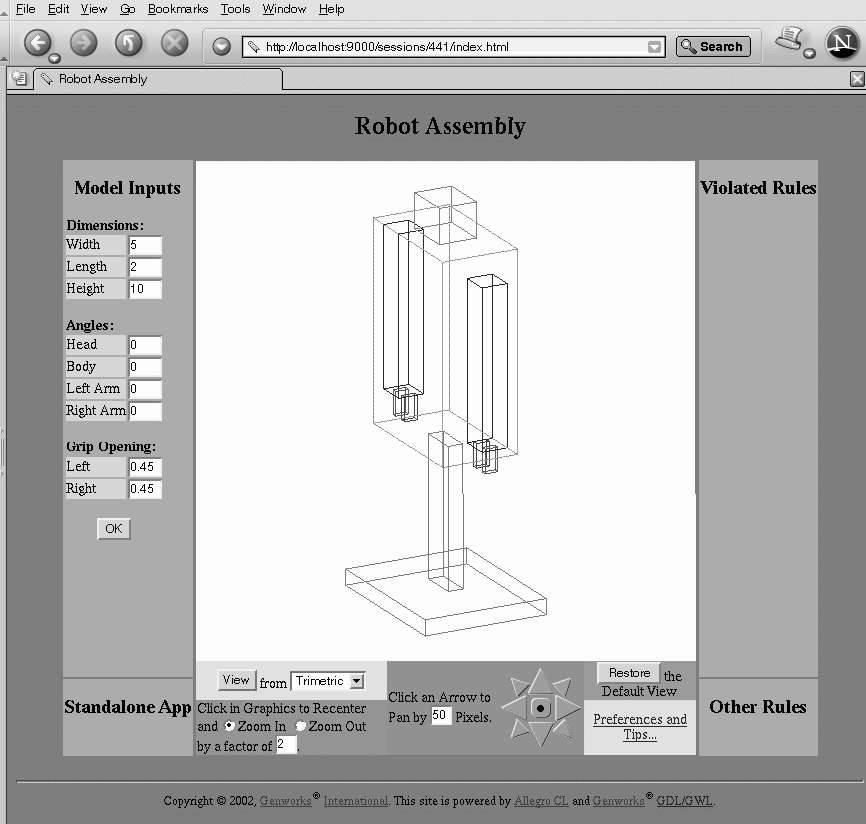
\includegraphics{../images/robot.png}
\end{center}

\caption{Default Robot}

\label{fig:robot}

\end{figure}


\section{Robot Geometry}

\label{sec:robotgeometry}

The actual robot is made up of two child objects, its \texttt{base} and its \texttt{body}, as shown in Figure 
\ref{code:robot-geometry-toplevel}. Figure 
\ref{code:robot-body} shows the definition of the body, and 
\ref{code:robot-base} shows the definition of the base. The body is made
up of a torso (a box), a head (a box), and two arms, whose
definition is shown in Figure 
\ref{code:robot-arm}. The \texttt{:settable} :computed-slots from the toplevel UI sheet come into the \texttt{robot} as input-slots. These serve as parameters for the rest of the robot hierarchy.

The positioning and orientation of each child object are specified by 
passing \texttt{\index{:center}:center} and \texttt{\index{:orientation}:orientation} into the child part:

\begin{description}

\item [:center]
is given as a 3D point, and causes the child object to treat this
point as its center.

\item [:orientation]
is given as a 3-by-3 rotational transformation matrix, and causes 
the child object to adjust its six \texttt{\index{face-normal-vector}face-normal-vector}s accordingly. As with this example, this transformation matrix is 
usually created using the \texttt{\index{alignment}alignment} function, which allows you to align up to three faces of the child
object with up to three given vectors. The first vector will be taken exactly, 
and the second and third vectors will be taken for their orthogonal components 
to the previous ones.

\end{description}


\begin{figure}
\begin{lrbox}{\boxedverb}
\begin{minipage}{\linewidth}
\small{

\begin{verbatim}


 (define-object robot (base-object)

   :input-slots
   (head-angle
    body-angle
    arm-angle-right
    arm-angle-left
    pincer-distance-right
    pincer-distance-left)

   :computed-slots
   ((display-controls (list :color :green-lime)))

   :objects
   ((base :type 'robot-base
          :height (* (the :height) 0.4)
          :width (* (the :width) 0.2)
          :length (* (the :length) 0.2)
          :center (translate (the :center) :down (* (the :height) 0.3)))
    (body :type 'robot-body
          :height (* (the :height) 0.6)
          :center (translate (the :center) :up (* (the :height) 0.2))
          :orientation 
          (alignment :right
                     (rotate-vector-d 
                      (the (:face-normal-vector :right))
                      (the :body-angle)
                      (the (:face-normal-vector :top))))
          :pass-down (:head-angle 
                      :arm-angle-right :arm-angle-left 
                      :pincer-distance-left :pincer-distance-right))))      
      
\end{verbatim}}
\end{minipage}
\end{lrbox}
\fbox{\usebox{\boxedverb}}

\caption{Toplevel of Robot Geometry}

\label{code:robot-geometry-toplevel}

\end{figure}

\begin{figure}
\begin{lrbox}{\boxedverb}
\begin{minipage}{\linewidth}
\small{

\begin{verbatim}


 (define-object robot-body (base-object)
   :input-slots
   (head-angle arm-angle-left arm-angle-right
    pincer-distance-left pincer-distance-right
    (shoulder-height (* (the :torso :height) 0.1)))

   :computed-slots
   ((display-controls (list :color :blue-steel-light)))

   :objects
   ((torso :type 'box :height (* (the :height) 0.85)
           :width (* (the :width) 0.7)
           :center (translate (the :center) 
                              :down (- (half (the :height)) 
                                       (half (the-child :height)))))
    (head :type 'box :display-controls (list :color :magenta)
          :height (- (the :height) (the :torso :height))
          :width (* (the :width) 0.25) :length (half (the :length))
          :center (translate (the :center) :up
                             (- (half (the :height)) (half (the-child :height))))
          :orientation (alignment :right
                                  (rotate-vector-d 
                                   (the (:face-normal-vector :right))
                                   (the :head-angle)
                                   (the (:face-normal-vector :top)))))
    (arms :type 'robot-arm :sequence (:size 2)
          :side (ecase (the-child :index) (0 :left) (1 :right))
          :width (half (- (the :width) (the :torso :width)))
          :length (/ (the :length) 3)
          :height (- (the :torso :height) (twice (the :shoulder-height)))
          :center (translate-along-vector 
                   (the-child :shoulder-point)
                   (the-child (:face-normal-vector :bottom)) 
                   (half (the-child :height)))
          :orientation 
          (alignment :bottom
                     (rotate-vector-d (the (:face-normal-vector :bottom))
                                      (the-child :angle)
                                      (the (:face-normal-vector :left)))
                     :right (the (:face-normal-vector :right)))
          :shoulder-point 
          (translate (the :torso (:edge-center :top (the-child :side)))
                     (the-child :side) (half (the-child :width)) :down
                     (the :shoulder-height))
          :angle (ecase (the-child :side) (:left (the :arm-angle-left))
                        (:right (the :arm-angle-right)))
          :pincer-distance (ecase (the-child :side) 
                             (:left (the :pincer-distance-left))
                             (:right (the :pincer-distance-right))))))
      
\end{verbatim}}
\end{minipage}
\end{lrbox}
\fbox{\usebox{\boxedverb}}

\caption{Robot Body}

\label{code:robot-body}

\end{figure}

\begin{figure}
\begin{lrbox}{\boxedverb}
\begin{minipage}{\linewidth}

\begin{verbatim}


 (define-object robot-arm (base-object)

   :input-slots
   (side
    shoulder-point
    angle
    pincer-distance)

   :computed-slots
   ((display-controls (list :color :blue)))

   :objects
   ((arm :type 'box)
    (thumb :type 'box
           :display-controls (list :color :red)
           :width (the :hand :width)
           :height (the :hand :height)
           :length (the :hand :length)
           :center (translate (the :hand :center) 
                              (the :side) (the :pincer-distance)))
    (hand :type 'box
          :display-controls (list :color :green)
          :center (translate (the :center) :down
                             (+ (half (the :height)) 
                                (half (the-child :height)))
                             (the :side)
                             (- (- (half (the :width)) 
                                   (half (the-child :width)))))
          :height (* (the :height) 0.15)
          :width (* (the :width) 0.2)
          :length (half (the :length)))))      
      
\end{verbatim}
\end{minipage}
\end{lrbox}
\fbox{\usebox{\boxedverb}}

\caption{Robot Arm}

\label{code:robot-arm}

\end{figure}

\begin{figure}
\begin{lrbox}{\boxedverb}
\begin{minipage}{\linewidth}

\begin{verbatim}


 (define-object robot-base (base-object)

   :objects
   ((leg :type 'box
         :height (* 0.9 (the :height))
         :center (translate (the :center) :up
                            (- (half (the :height)) 
                               (half (the-child :height)))))
    (foot :type 'box
          :height (* 0.1 (the :height))
          :width (twice (twice (the :width)))
          :length (twice (twice (twice (the :length))))
          :center (translate (the :center) :down
                             (- (half (the :height)) 
                                (half (the-child :height)))))))      
      
\end{verbatim}
\end{minipage}
\end{lrbox}
\fbox{\usebox{\boxedverb}}

\caption{Robot Base}

\label{code:robot-base}

\end{figure}


\section{Using the App}

\label{sec:usingtheapp}

Figures 
\ref{fig:robot-front} and 
\ref{fig:robot-swing} show some examples of a user having interacted with the application, resulting in
a specified standard 3D view of the robot or the robot's body parts rotated to specified
angles. Note also the extra hyperlinks at the upper-left in Figure 
\ref{fig:robot-front}, which are a result of the GDL/GWL session being in \emph{\index{development mode}development mode}. Development mode can be entered as follows:\index{gwl:*developing?*}

\begin{verbatim}(setq gwl:*developing?* t)
\end{verbatim}The three standard links provided by development mode are as follows:

\begin{description}

\item [Update!]
will essentially re-instantiate the object hierarchy from the current object downward, taking into account any new or altered
definitions you have compiled since the objects were last demanded. However, any \texttt{:settable} slots which have been altered will retain their values to the extent feasible.

\item [Full Update!]
will perform and Update all the way from the root object.

\item [Break]
will cause a Common Lisp break level to be entered, with the parameter \texttt{self} set to the object instance corresponding to the current web page.

\item [\index{TaTu}TaTu]
will respond with the development view of the object, as described in the file \texttt{tatu.txt}.

\end{description}


\begin{figure}
\begin{center}
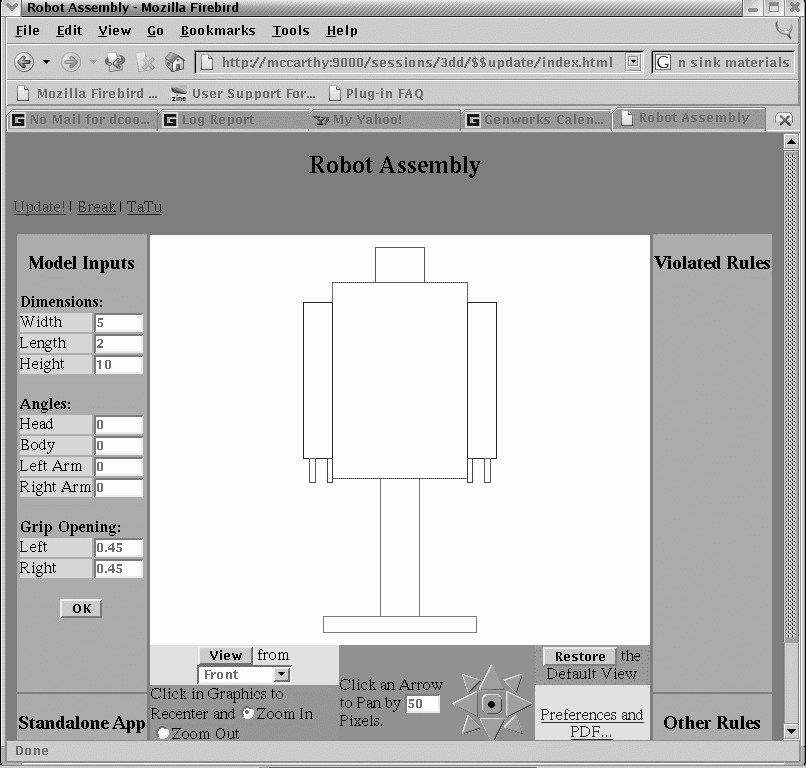
\includegraphics{../images/robot-front.png}
\end{center}

\caption{Front View of Robot}

\label{fig:robot-front}

\end{figure}

\begin{figure}
\begin{center}
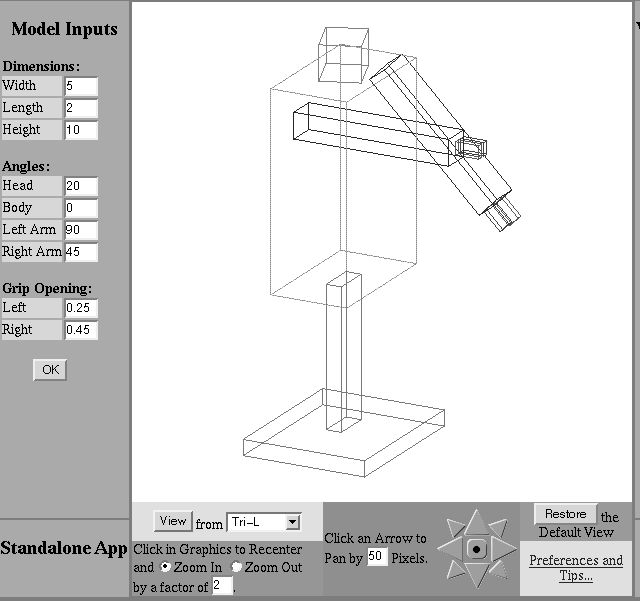
\includegraphics{../images/robot-swing.png}
\end{center}

\caption{Robot with some non-Default Angles}

\label{fig:robot-swing}

\end{figure}


\chapter{Example 3: School Bus}

\label{chap:example3:schoolbus}

In this chapter we leave you with another example of a geometric
GDL/GWL application, heavy on code examples, with a bit of explanation
sprinkled in between. This School Bus example introduces the use of
the \texttt{\index{node-mixin}node-mixin} primitive object, which is similar to \texttt{\index{application-mixin}application-mixin} which we met in the last chapter. But \texttt{node-mixin} is used to \emph{contain} other instances of either \texttt{node-mixin} or \texttt{application-mixin}, and automatically collects up any \texttt{\index{ui-display-list-objects}ui-display-list-objects} or rule objects (i.e.\ objects of type \texttt{\index{gwl-rule-object}gwl-rule-object}) from its descendants.

\section{Toplevel Assembly}

\label{sec:toplevelassembly}

Figure 
\ref{code:school-bus} defines the toplevel assembly consisting of a chassis, body, and interior. 

The toplevel mixes in \texttt{node-mixin}, and the chassis, body, and interior each mix in \texttt{application-mixin}. This results in a high-level user-visible hierarchy, shown as 
the ``Assembly Tree'' in the lower-left of Figure 
\ref{fig:school-bus}. Note that there is no need to specify a \texttt{ui-display-list-objects} slot in the \texttt{assembly}. This is because \texttt{node-mixin} automatically defines this slot, which appends together the \texttt{ui-display-list-objects} from any child objects of appropriate types.
       
Three toplevel \texttt{:settable} computed-slots are also specified, affecting the overall dimensions of the vehicle. 

Figure 
\ref{code:school-bus-model-inputs} defines the \texttt{model-inputs} for the toplevel, corresponding to the three \texttt{:settable} computed-slots in the \texttt{assembly}. 

The complete code for the School Bus example is provided on the GDL (and Trial Edition) CD;
in this tutorial we provide only the major portion of the interior. The chassis and body are 
defined similarly, although the chassis in particular contains several interesting examples,
which are beyond the scope of this tutorial, of solving somewhat ``heavier'' engineering 
problems with GDL/GWL.
\begin{figure}
\begin{lrbox}{\boxedverb}
\begin{minipage}{\linewidth}

\begin{verbatim}


 (define-object assembly (node-mixin)

   :computed-slots
   ((frame-datum (let ((datum
                        (read-safe-string (string-append
                                           "("
                                           (the frame-datum-m)
                                           ")"))))
                   (translate (the center) :right (first datum) :rear
                              (second datum) :top (third datum))))
    (strings-for-display "School Bus")
    (wheelbase 300 :settable)
    (track 96 :settable)
    (height 80 :settable)
    (frame-datum-m "2000 500 0" :settable))

   :objects
   ((chassis :type 'chassis
             :pass-down (:wheelbase :track)
             :datum (the frame-datum)
             :height 20)
    (body :type 'body
          :pass-down (:wheelbase :track)
          :frame-width (the chassis frame-width)
          :frame-overhang (- (the-child front-overhang) 
                             (the chassis front-overhang))
          :firewall-base (translate 
                          (the frame-datum) :up
                          (half (the chassis frame-height)) :right
                          (- (the-child cab-width)
                             (the-child frame-overhang))))
    (interior :type 'interior
              :firewall-base (the body firewall-base)
              :width (- (the body width) (the body cab-width))
              :length (the body length)
              :height (the body height))))

\end{verbatim}
\end{minipage}
\end{lrbox}
\fbox{\usebox{\boxedverb}}

\caption{Toplevel Assembly for School Bus}

\label{code:school-bus}

\end{figure}

\begin{figure}
\begin{lrbox}{\boxedverb}
\begin{minipage}{\linewidth}

\begin{verbatim}


 (define-view (html-format assembly) nil
  
   :output-functions
   ((model-inputs
     nil
     (html 
      (:p
       (:table
        (:tr ((:td :bgcolor :yellow) "Wheelbase")
             (:td
              ((:input :type :text :size 5 :name :wheelbase :value
                       (the :wheelbase)))))
        (:tr ((:td :bgcolor :yellow) "Track")
             (:td ((:input :type :text :size 5 
                           :name :track :value (the :track)))))
        (:tr ((:td :bgcolor :yellow) "Height")
             (:td
              ((:input :type :text :size 5 
                       :name :height :value (the :height)))))))
      (:p ((:input :type :submit :name :submit :value " OK ")))))))

\end{verbatim}
\end{minipage}
\end{lrbox}
\fbox{\usebox{\boxedverb}}

\caption{HTML format View of Model Inputs for School Bus Toplevel}

\label{code:school-bus-model-inputs}

\end{figure}

\begin{figure}
\begin{center}
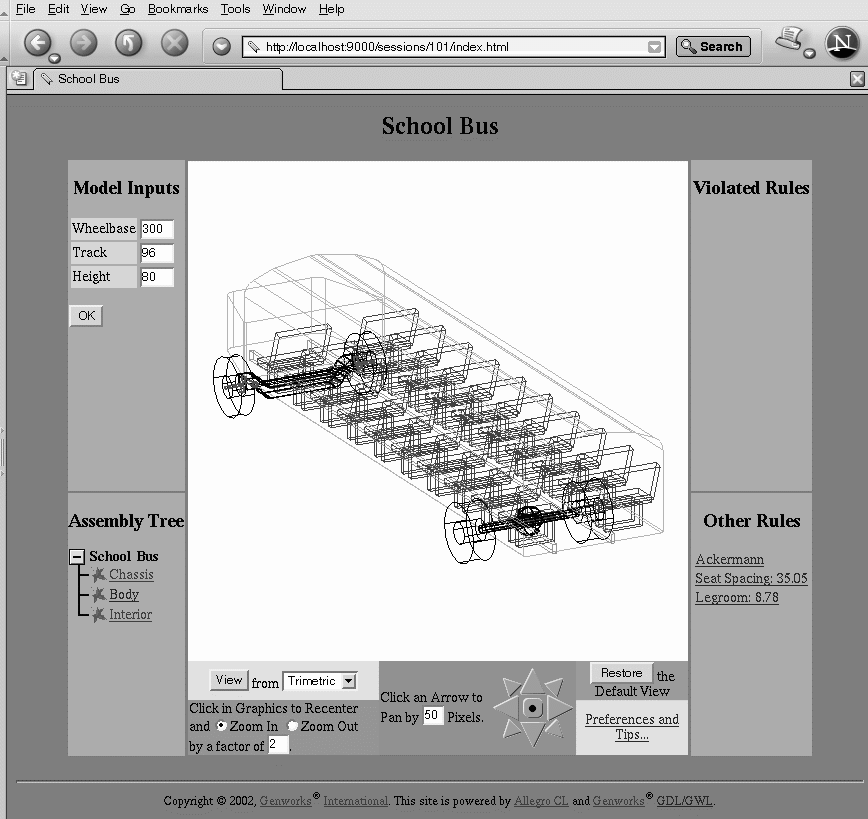
\includegraphics{../images/school-bus.png}
\end{center}

\caption{Toplevel Sheet of School Bus App}

\label{fig:school-bus}

\end{figure}


\section{Interior of School Bus}

\label{sec:interiorofschoolbus}

Figures 
\ref{code:school-bus-interior} and 
\ref{code:school-bus-seating-section} define the major components making up the interior of the bus, which for our
current purposes consists of the bench seats and a few rules regarding their 
spacing.

In particular, Figure 
\ref{code:school-bus-seating-section} defines the \texttt{seating-section} which contains the two actual columns of bench seats. This object also contains
two \emph{rule objects} which compute certain key pieces of information:

\begin{description}

\item [inter-seat-spacing-computation]
computes the exact spacing from the front of one seat to the front of the next,
given the available cabin width (i.e.\ coach length), the maximumm allowed recline angle
of the seat backs, and the number of rows to be fit into the bus. (The actual seat 
dimensions are taken from defaults in the seat object definition, not listed here).

This spacing value is crucial for two reasons: first, this value is used in order to 
generate the actual geometric objects that you see in the graphical output. Second,
this value is used in the \texttt{inter-seat-clearance-check} to compare with the overall length of one seat, to compute how much is 
left over to be considered ``legroom.''
\index{rules!diagnostic}\index{rules!generative}\index{rules!violating}\index{rules!model!tight integration with}\index{rules}
\item [inter-seat-clearance-check]
is a purely diagnostic rule which uses values from the spacing computation
rule in order to compute the effective ``legroom'' between seats. This legroom
is compared with the rule's specified \texttt{value} (in this case representing the allowed minimum value), to determine whether the rule
has violated its condition or not.

\end{description}

It is typical in a KB model to have this kind of tight integration between
``rules'' and the model itself --- when an input to the model is changed, any
rules and other objects which directly or indirectly depend on that input will 
automatically re-evaluate themselves. Rules and objects which are not affected 
by a given change will avoid the computational work of re-evaluating themselves. 

Maintaining this kind of dependency management in a traditional
procedural language environment becomes extremely burdensome on the
application developer. In a KB environment, however, this dependency
management ``just happens'' as a matter of course.\index{dependency management}
\begin{figure}
\begin{lrbox}{\boxedverb}
\begin{minipage}{\linewidth}

\begin{verbatim}


 (define-object interior (application-mixin)

   :input-slots
   (firewall-base
    length
    width
    height)

   :computed-slots
   ((ui-display-list-objects (the :sections))
    (number-of-rows 10 :settable)
    (reclined-angle 20 :settable)
    (max-reclined-angle 30 :settable)
    (minimum-inter-seat-clearance 7 :settable))

   :objects
   ((sections :type 'seating-section
              :body-reference-points 
              (list :left
                    (translate (the :firewall-base) :front
                               (half (the :length)) :right
                               (the :width))
                    :right
                    (translate (the :firewall-base) :rear
                               (half (the :length)) :right
                               (the :width)))
              :usable-cabin-width (the :width)
              :pass-down (:number-of-rows 
                          :reclined-angle :max-reclined-angle
                          :minimum-inter-seat-clearance))))      
      
\end{verbatim}
\end{minipage}
\end{lrbox}
\fbox{\usebox{\boxedverb}}

\caption{Interior Assembly Component School Bus}

\label{code:school-bus-interior}

\end{figure}

\begin{figure}
\begin{lrbox}{\boxedverb}
\begin{minipage}{\linewidth}

\begin{verbatim}


 (define-view (html-format interior) nil

   :output-functions
   ((model-inputs
     nil
     (html 
      (:p
       (:table
        (:tr 
         ((:td :bgcolor :yellow) "Rows")
         (:td
          ((:input :type :text :size 5 
                   :name :number-of-rows :value
                   (the :number-of-rows)))))
        (:tr 
         ((:td :bgcolor :yellow) "Seat Recline")
         (:td
          ((:input :type :text :size 5 
                   :name :reclined-angle :value
                   (the :reclined-angle)))))
        (:tr 
         ((:td :bgcolor :yellow) "Max Recline")
         (:td
          ((:input :type :text :size 5 
                   :name :max-reclined-angle :value
                   (the :max-reclined-angle)))))
        (:tr 
         ((:td :bgcolor :yellow) "Req'd Clearance")
         (:td
          ((:input :type :text :size 5 
                   :name :minimum-inter-seat-clearance
                   :value (the :minimum-inter-seat-clearance)))))))
      (:p ((:input :type :submit :name :submit :value " OK ")))))))      
      
\end{verbatim}
\end{minipage}
\end{lrbox}
\fbox{\usebox{\boxedverb}}

\caption{HTML Format Model Inputs of School Bus Interior}

\label{code:school-bus-interior-model-inputs}

\end{figure}

\begin{figure}
\begin{center}
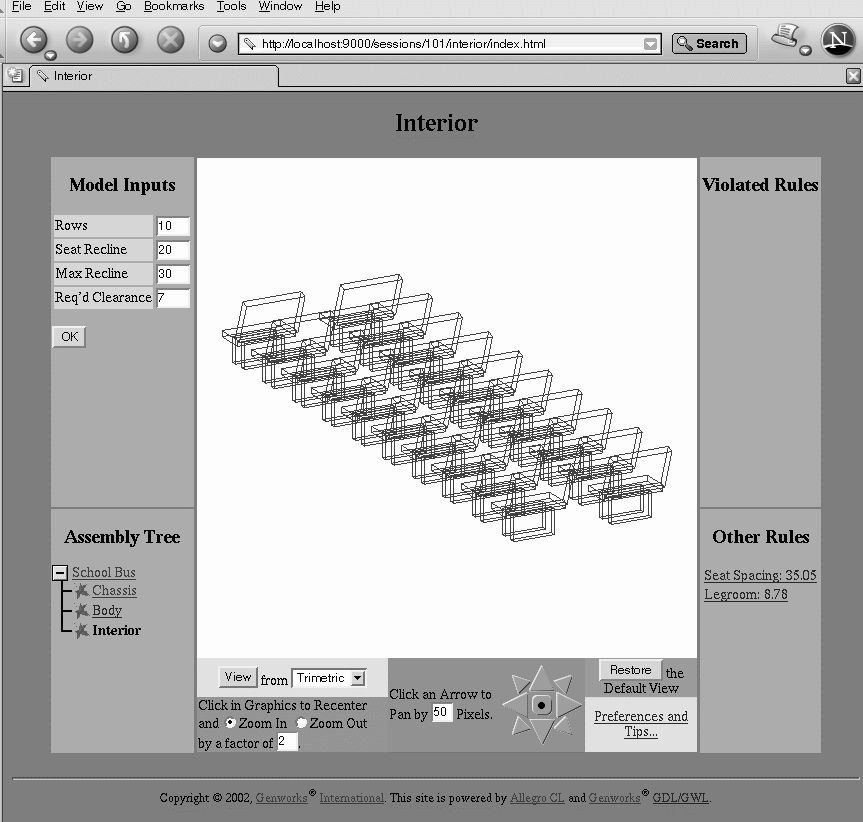
\includegraphics{../images/school-bus-interior.png}
\end{center}

\caption{Interior of School Bus}

\label{fig:school-bus-interior}

\end{figure}

\begin{figure}
\begin{lrbox}{\boxedverb}
\begin{minipage}{\linewidth}

\begin{verbatim}


 (define-object seating-section (base-object)

   :input-slots
   (fare-class
    usable-cabin-width
    body-reference-points
    max-reclined-angle
    number-of-rows
    minimum-inter-seat-clearance)

   :objects
   ((inter-seat-spacing-computation 
     :type 'inter-seat-spacing
     :pass-down (:max-reclined-angle 
                 :usable-cabin-width :number-of-rows))
    (inter-seat-clearance-check 
     :type 'inter-seat-clearance-check
     :inter-seat-spacing (the inter-seat-spacing-computation result)
     :clearance-extent-typical (the inter-seat-spacing-computation
                                 clearance-extent-typical)
     :value (the minimum-inter-seat-clearance))
    (sides :type 'seating-side
           :fare-class (the fare-class)
           :sequence (:size 2)
           :side (ecase (the-child index) (0 :left) (1 :right))
           :display-controls (list :color :green)
           :body-reference-point (getf (the body-reference-points) 
                                       (the-child side))
           :pass-down (:number-of-rows :reclined-angle)
           :inter-seat-spacing 
           (the inter-seat-spacing-computation result)
           :x-max-typical 
           (the inter-seat-spacing-computation x-max-typical)
           :x-vector (the (face-normal-vector :right)))))
      
\end{verbatim}
\end{minipage}
\end{lrbox}
\fbox{\usebox{\boxedverb}}

\caption{Object Definition for Seating Columns}

\label{code:school-bus-seating-section}

\end{figure}

\begin{figure}
\begin{center}
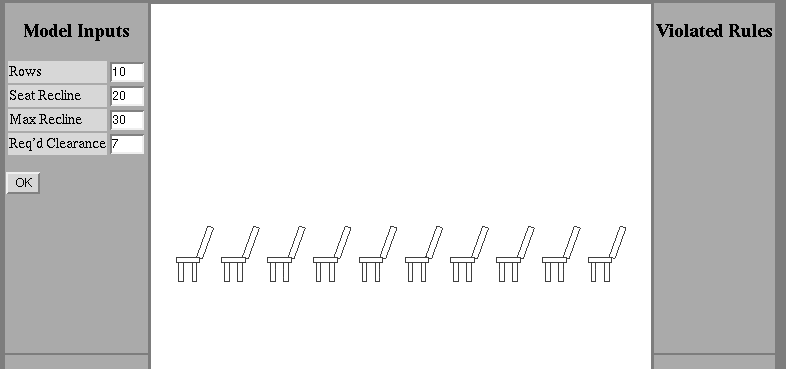
\includegraphics{../images/school-bus-interior-front.png}
\end{center}

\caption{Front View of School Bus Interior}

\label{fig:school-bus-interior-front}

\end{figure}


\newpage



\section{Causing a Rule Violation}

\label{sec:causingaruleviolation}

Figure 
\ref{fig:school-bus-violated} shows the state of the interior after a user has changed the number of seating
rows to eleven, from the default ten. The user has also changed the displayed recline 
angle of the seat backs to match the maximum allowed value (30 degrees). 

In this state, the seats have redistributed themselves so that they
still are spaced evenly in the available length of the coach. However,
this has caused a violation in the legroom, defined as the horizontal
distance from the rear-center of one seat back to the front of the
seat bottom aft of it. The allowed value for this legroom (``Req'd
Clearance'') is 7, and the current legroom value (as computed by
the rule object) is now less than this.

Therefore we have a violation, and the link to the rule shows up in
the ``Violations'' section of the user interface.

For a typical example such as this School Bus, one can imagine
dozens or hundreds of other rules. Many such rules can be computed
based on information we already have in our model, and others will
result in the model being augmented incrementally with new information
as needed.

The main point is that we now have a stable, user-friendly, and
readily scalable framework in which to represent and grow 
our ``knowledge.''


\begin{figure}
\begin{center}
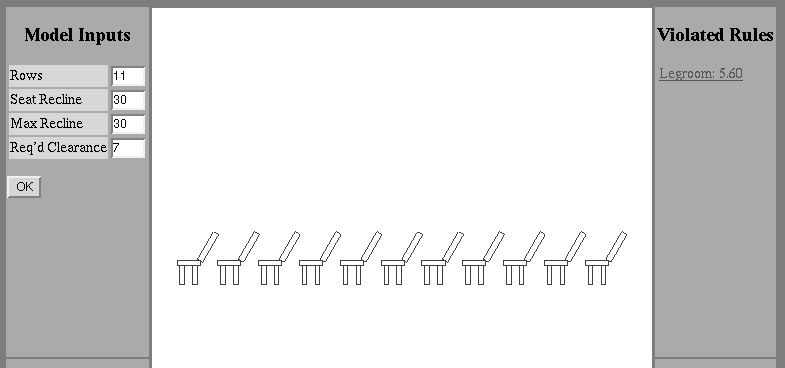
\includegraphics{../images/school-bus-interior-violated.png}
\end{center}

\caption{Interior of School Bus with 11 Rows (Legroom Violation)}

\label{fig:school-bus-violated}

\end{figure}


\backmatter



\printindex



\end{document}

